\subsection{EXTENSION OF THE RING OF SCALARS OF A MODULE}

Let A, B be two rings and \(\rho: \mathbf{A} \to \mathbf{B}\) a ring homomorphism; we consider the right A-module \(\rho^{*}(B_{d})\) defined by this homomorphism (§ 1, no. 13); this A-module also has a left B-module structure, namely that of \(B_{s}\) and, as \(b'(b\rho(a)) = (b'b)\rho(a)\) for \(a \in \mathbf{A}\) , \(b\) , \(b'\) in B, these two module structures on B are compatible (§ 1, no. 14). This allows us, for every left A-module E, to define a left B-module structure on the tensor product \(\rho_{*}(B_{d}) \otimes_{\mathbf{A}} \mathbf{E}\) such that \(\beta'(\beta \otimes x) = (\beta'\beta) \otimes x\) for \(\beta\) , \(\beta'\) in B and \(x \in \mathbf{E}\) (§ 3, no. 3). This left B-module is said to be derived from E by extending the ring of scalars to B by means of \(\rho\) and it is denoted by \(\rho^{*}(\mathbf{E})\) or \(\mathrm{E}_{(\mathbf{B})}\) if no confusion arises.

PROPOSITION 1. For every left A-module E, the mapping \(\phi: x \mapsto 1 \otimes x\) of E into the A-module \(\rho_*(\rho^*(\mathbf{E}))\) is A-linear and the set \(\phi(\mathbf{E})\) generates the B-module \(\rho^*(\mathbf{E})\) . Further, for every left B-module F and every A-linear mapping \(f\) of E into the A-module \(\rho_*(\mathbf{F})\) , there exists one and only one B-linear mapping \(\tilde{f}\) of \(\rho^*(\mathbf{E})\) into F such that \(\tilde{f}(1 \otimes x) = f(x)\) for all \(x \in \mathbf{E}\) .

B can be considered as a (B, A)-bimodule by means of \(\rho\) ; then there is a canonical Z-module isomorphism

\[
\operatorname{Hom} _ {\mathbf {B}} (\mathbf {B} \otimes_ {\mathbf {A}} \mathbf {E}, \mathbf {F}) \rightarrow \operatorname{Hom} _ {\mathbf {A}} (\mathbf {E}, \operatorname{Hom} _ {\mathbf {B}} (\mathbf {B} _ {s}, \mathbf {F}))\tag{1}
\]

as has been seen in § 4, no. 1, Proposition 1. But the left A-module \(\mathrm{Hom}_{\mathbf{B}}(\mathbf{B}_{s},\mathbf{F})\) is canonically identified with \(\rho^{*}(\mathbf{F})\) : for, by definition (§ 1, no. 14), there corresponds to an element \(y\in \mathbf{F}\) the homomorphism \(\theta (y)\colon \mathbf{B}_s\to \mathbf{F}\) such that \((\theta (y))(1) = y\) ; for all \(\lambda \in \mathbf{A}\) , there thus corresponds to \(\rho (\lambda)y\in \mathbf{F}\) the homomorphism \(\mu \mapsto \mu \rho (\lambda)y\) of \(\mathbf{B}_s\) into \(\mathbf{F}\) , which is just \(\lambda \theta (y)\) for the left A-module structure on \(\mathrm{Hom}_{\mathbf{B}}(\mathbf{B}_{s},\mathbf{F})\) (§ 1, no. 14). Using this identification, we obtain therefore a canonical Z-module isomorphism, the inverse of (1)

\[
\delta : \operatorname{Hom} _ {\mathbf {A}} (\mathbf {E}, \rho_ {*} (\mathbf {F})) \rightarrow \operatorname{Hom} _ {\mathbf {B}} (\rho^ {*} (\mathbf {E}), \mathbf {F})\tag{2}
\]

and it follows immediately from the definitions that if \(\delta(f) = \bar{f}\) then \(\bar{f}(1 \otimes x) = f(x)\) for all \(x \in \mathbf{E}\) . In particular, the mapping \(\phi_{\mathbb{E}}: x \mapsto 1 \otimes x\) is just

\[
\phi_ {\mathbf {E}} = \delta^ {- 1} (1 _ {\rho^ {*} (\mathbf {E})}).\tag{3}
\]

Proposition 1 is therefore proved. The mapping \(\phi_{\mathbf{E}}: \mathbf{E} \to \rho_{*}(\rho^{*}(\mathbf{E}))\) is called canonical.

Remarks. (1) Proposition 1 shows that the ordered pair consisting of \(\mathbf{E}_{(\mathbf{B})}\) and \(\phi_{\mathbb{E}}\) is a solution of the universal mapping problem (Set Theory, IV, §3, no. 1), where \(\Sigma\) is the species of left B-module structures (the morphisms being B-linear mappings) and the \(\alpha\) -mappings are the A-linear mappings of E into a B-module.

\begin{enumerate}
\def\labelenumi{(\arabic{enumi})}
\setcounter{enumi}{1}
\item
  If E is an \((\mathbf{A}, (\mathbf{C}_{i}^{\prime}); (\mathbf{D}_{j}^{\prime}))\) -multimodule and F a \((\mathbf{B}, (\mathbf{C}_{h}^{\prime\prime}); (\mathbf{D}_{k}^{\prime\prime}))\) -multimodule, then the isomorphism (2) is linear with respect to the \(((\mathbf{D}_{j}^{\prime}), (\mathbf{C}_{h}^{\prime\prime}); (\mathbf{C}_{i}^{\prime}), (\mathbf{D}_{k}^{\prime\prime}))\) -multimodule structures of the two sides (§ 1, no. 14 and § 3, no. 4).
\item
  Let E be a left A-module, a a two-sided ideal of A and \(\rho:A\to A/a\) the canonical homomorphism. In the notation of §3, no. 6, Corollary 2 to Proposition 6, the A-module E/aE is annihilated by a and therefore has canonically a left (A/a)-module structure (§1, no. 12); it is immediate that the canonical mapping \(\pi:\rho^{*}(E)\to E/aE\) defined in §3, no. 6, Corollary 2 to Proposition 6 is an isomorphism for the (A/a)-module structures.
\end{enumerate}

COROLLARY. Let E, E' be two left A-modules; for every A-linear mapping u: E → E', v = l\_B ⊗ u is the unique B-linear mapping which renders commutative the diagram

\pandocbounded{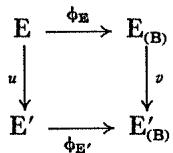
\includegraphics[keepaspectratio]{images/part002_74d11806.jpg}}

where \(\phi_{\mathbf{E}}\) and \(\phi_{\mathbf{E}'}\) are the canonical mappings.

It suffices to apply Proposition 1 to the A-homomorphism \(\phi_{\mathbf{E}'} \circ u: \mathbf{E} \to \mathbf{E}_{(\mathbf{B})}'\) .

The mapping \(v\) defined in the above corollary is denoted by \(\rho^{*}(u)\) or \(u_{(B)}\) . If \(E''\) is a third left A-module and \(v: E' \to E''\) an A-linear mapping, it is immediate that

\[
\left(v \circ u\right) _ {(\mathbf {B})} = v _ {(\mathbf {B})} \circ u _ {(\mathbf {B})}.
\]

Extending the ring of operators of a module is a transitive operation; to be precise:

PROPOSITION 2. Let \(\rho: \mathbf{A} \to \mathbf{B}\) , \(\sigma: \mathbf{B} \to \mathbf{C}\) be ring homomorphisms. For every left A-module E, there exists one and only one C-homomorphism

\[
\sigma^ {*} (\rho^ {*} (\mathrm{E})) \rightarrow (\sigma \circ \rho) ^ {*} (\mathrm{E})\tag{4}
\]

mapping \(1 \otimes (1 \otimes x)\) to \(1 \otimes x\) for all \(x \in E\) and this homomorphism is bijective.

The underlying Z-modules of \(\sigma^{*}(\rho^{*}(\mathbf{E}))\) and \((\sigma \circ \rho)^{*}(\mathbf{E})\) are respectively \(\mathbf{C} \otimes_{\mathbf{B}} (\mathbf{B} \otimes_{\mathbf{A}} \mathbf{E})\) and \(\mathbf{C} \otimes_{\mathbf{A}} \mathbf{E}\) . There exists a canonical Z-isomorphism \(\mathbf{C} \otimes_{\mathbf{B}} (\mathbf{B} \otimes_{\mathbf{A}} \mathbf{E}) \to (\mathbf{C} \otimes_{\mathbf{B}} \mathbf{B}) \otimes_{\mathbf{A}} \mathbf{E}\) (§ 3, no. 8, Proposition 8), which is also a C-isomorphism for the left C-module structures on both sides. Moreover, the C-module C ⊗B B is canonically identified with the C-module Cs under the isomorphism which maps γ ⊗ β to γσ(β) (§ 3, no. 4, Proposition 4) and this isomorphism is also an isomorphism for the right A-module structure on C ⊗B B defined by ρ and the right A-module structure on C defined by σ ∘ ρ. Thus a canonical isomorphism

\[
(\mathbf {C} \otimes_ {\mathbf {B}} \mathbf {B}) \otimes_ {\mathbf {A}} \mathbf {E} \rightarrow \mathbf {C} \otimes_ {\mathbf {A}} \mathbf {E}
\]

is obtained and, composing it with the isomorphism

\[
\mathbf {C} \otimes_ {\mathbf {B}} (\mathbf {B} \otimes_ {\mathbf {A}} \mathbf {E}) \rightarrow (\mathbf {C} \otimes_ {\mathbf {B}} \mathbf {B}) \otimes_ {\mathbf {A}} \mathbf {E}
\]

defined earlier, the desired canonical isomorphism is obtained.

If \(\phi, \phi'\) and \(\phi''\) denote the canonical mappings \(E \to \rho^*(E)\) , \(\rho^*(E \to) \sigma^*(\rho^*(E))\) and \(E \to (\sigma \circ \rho)^*(E)\) , \(\phi' \circ \phi\) is identified with \(\phi''\) under the canonical isomorphism of Proposition 2.

PROPOSITION 3. Let A, B be two commutative rings, \(\rho: \mathbf{A} \to \mathbf{B}\) a ring homomorphism and E, E' two A-modules. There exists one and only one B-homomorphism

\[
\mathbf {E} _ {(\mathbf {B})} \otimes_ {\mathbf {B}} \mathbf {E} _ {(\mathbf {B})} ^ {\prime} \rightarrow (\mathbf {E} \otimes_ {\mathbf {A}} \mathbf {E} ^ {\prime}) _ {(\mathbf {B})}\tag{5}
\]

mapping \((1 \otimes x) \otimes (1 \otimes x')\) to \(1 \otimes (x \otimes x')\) for \(x \in \mathbf{E}\) , \(x' \in \mathbf{E}'\) , and this homomorphism is bijective.

The left hand side of (5) may be written \((\mathbf{B} \otimes_{\mathbf{A}} \mathbf{E}) \otimes_{\mathbf{B}} (\mathbf{B} \otimes_{\mathbf{A}} \mathbf{E}')\) and is identified with \((\mathbf{E} \otimes_{\mathbf{A}} \mathbf{B}) \otimes_{\mathbf{B}} (\mathbf{B} \otimes_{\mathbf{A}} \mathbf{E}')\) since A and B are commutative; the latter product is identified successively with \(\mathbf{E} \otimes_{\mathbf{A}} (\mathbf{B} \otimes_{\mathbf{B}} \mathbf{B}) \otimes_{\mathbf{A}} \mathbf{E}'\) , \(\mathbf{E} \otimes_{\mathbf{A}} (\mathbf{B} \otimes_{\mathbf{A}} \mathbf{E}')\) , \(\mathbf{E} \otimes_{\mathbf{A}} (\mathbf{E}' \otimes_{\mathbf{A}} \mathbf{B})\) and finally \((\mathbf{E} \otimes_{\mathbf{A}} \mathbf{E}') \otimes_{\mathbf{A}} \mathbf{B}\) , using the associativity of the tensor product (§ 3, no. 8, Proposition 8), Proposition 4, § 3, no. 4, and the commutativity of A and B. The desired isomorphism is the composition of the successive canonical isomorphisms.

Clearly if S is a generating system of E, the image of S under the canonical mapping \(E \rightarrow E_{(B)}\) is a generating system of \(E_{(B)}\) ; in particular, if E is a finitely generated A-module, \(E_{(B)}\) is a finitely generated B-module.

PROPOSITION 4. Let E be an A-module admitting a basis \((a_{\lambda})_{\lambda \in L}\) ; if \(\phi : x \mapsto 1 \otimes x\) is the canonical mapping of E into \(\rho^{*}(\mathbf{E})\) , then \((\phi(a_{\lambda}))_{\lambda \in L}\) is a basis of \(\rho^{*}(\mathbf{E})\) . If \(\rho\) is injective, so is \(\phi\) .

The first assertion follows immediately from § 3, no. 7, Corollary 1 to Proposition 7. Also, for every family \((\xi_{\lambda})_{\lambda \in L}\) of elements of A of finite support, \(\phi\left(\sum_{\lambda \in L} \xi_{\lambda} a_{\lambda}\right) = \sum_{\lambda \in L} \rho(\xi_{\lambda}) \phi(a_{\lambda})\) and the relation \(\phi\left(\sum_{\lambda \in L} \xi_{\lambda} a_{\lambda}\right) = 0\) is therefore equivalent to \(\rho(\xi_{\lambda}) = 0\) for all \(\lambda \in L\) , whence the second assertion.

COROLLARY. For every projective A-module E, the B-module \(\rho^{*}(\mathbf{E})\) is projective. If further \(\rho\) is injective, the canonical mapping of E into \(\rho^{*}(\mathbf{E})\) is injective.

By hypothesis there exists a free A-module M containing E and in which E admits a supplement F. It follows immediately from §3, no. 7, Proposition 7 that \(\mathbf{M}_{(\mathbf{B})}\) is identified with the direct sum of \(\mathbf{E}_{(\mathbf{B})}\) and \(\mathbf{F}_{(\mathbf{B})}\) and if \(\phi\) and \(\psi\) are the canonical mappings \(\mathbf{E} \to \mathbf{E}_{(\mathbf{B})}\) and \(\mathbf{F} \to \mathbf{F}_{(\mathbf{B})}\) , the canonical mapping \(\mathbf{M} \to \mathbf{M}_{(\mathbf{B})}\) is just \(x + y \mapsto \phi(x) + \psi(y)\) . The corollary follows immediately from Proposition 4 applied to the A-module M.

When E is a right A-module, we write similarly \(\rho^{*}(\mathbf{E}) = \mathbf{E} \otimes_{\mathbf{A}} \rho_{*}(\mathbf{B}_{s})\) , B being considered this time as an (A, B)-bimodule and the right B-module structure on \(\rho^{*}(\mathbf{E})\) being such that \((x \otimes \beta)\beta' = x \otimes (\beta\beta')\) for \(\beta \in B, \beta' \in B\) and \(x \in E\) . We leave to the reader the task of stating for right modules the results corresponding to those of this no. and the following.

Remark (4). Consider the left A-module \(\rho_{*}(B_{s})\) defined by \(\rho\) and for every left A-module E, consider the Z-module

\[
\tilde {\rho} (\mathbf {E}) = \operatorname{Hom} _ {\mathbf {A}} \left(\rho_ {*} \left(\mathbf {B} _ {s}\right), \mathbf {E}\right).\tag{6}
\]

As \(\rho_{*}(\mathbf{B}_{s})\) has a right B-module structure, a left B-module structure is derived on \(\tilde{\rho}(\mathbf{E})\) ( \(\S 1\) , no. 14) such that, if \(u \in \tilde{\rho}(\mathbf{E})\) and \(b' \in \mathbf{B}\) , \(b'u\) is the homomorphism \(b \mapsto u(bb')\) of \(\rho_{*}(\mathbf{B}_{s})\) into \(\mathbf{E}\) . We further define an A-linear mapping, called canonical

\[
\eta : \rho_ {*} (\tilde {\rho} (\mathbf {E})) \rightarrow \mathbf {E}\tag{7}
\]

associating with every homomorphism \(u \in \tilde{\rho}(\mathbf{E})\) the element \(u(1)\) in \(\mathbf{E}\) . As \(\mathbf{B}\) can be considered as an (A, B)-bimodule by means of \(\rho\) , for every left B-module \(\mathbf{F}\) , there is a canonical \(\mathbf{Z}\) -module isomorphism

\[
\operatorname{Hom} _ {\mathbf {A}} \left(\rho_ {*} (\mathrm{B} _ {s}) \otimes_ {\mathrm{B}} \mathrm{F}, \mathrm{E}\right)\rightarrow \operatorname{Hom} _ {\mathbf {B}} (\mathrm{F}, \operatorname{Hom} _ {\mathbf {A}} \left(\rho_ {*} (\mathrm{B} _ {s}), \mathrm{E}\right))
\]

(§ 1, no. 1, Proposition 1). As the left A-module \(\rho^{*}(B_{s}) \otimes_{B} F\) is canonically identified with \(\rho_{*}(F)\) by virtue of § 3, no. 4, Proposition 4, we obtain a canonical Z-module isomorphism, the inverse of the above

\[
\operatorname{Hom} _ {\mathbf {B}} (\mathbf {F}, \tilde {\rho} (\mathbf {E})) \rightarrow \operatorname{Hom} _ {\mathbf {A}} (\rho_ {*} (\mathbf {F}), \mathbf {E})\tag{8}
\]

which associates with every B-linear mapping g of F into \(\tilde{\rho}(\mathbf{E})\) the composite mapping \(\eta \circ g\) , considered as an A-linear mapping of \(\rho_{*}(\mathbf{F})\) into E. In particular, under the hypotheses of Proposition 2, if F is replaced by \(\sigma_{*}(\mathbf{C}_{s})\) , we obtain a canonical C-isomorphism

\[
\tilde {\sigma} (\tilde {\rho} (\mathbf {E})) \rightarrow (\sigma \circ \rho) ^ {\sim} (\mathbf {E}).\tag{9}
\]

